\documentclass[12pt]{article}
\usepackage[margin=3cm]{geometry}
\usepackage{graphicx}
\usepackage{float}
\usepackage{url}
\usepackage{listings}
\usepackage{color}

\definecolor{mygreen}{rgb}{0,0.6,0}
\definecolor{mygray}{rgb}{0.5,0.5,0.5}
\definecolor{mymauve}{rgb}{0.58,0,0.82}
\lstset{ %
	xleftmargin=2em,
	backgroundcolor=\color{white},   % choose the background color; you must add \usepackage{color} or \usepackage{xcolor}
	basicstyle=\small,%\footnotesize,        % the size of the fonts that are used for the code
	breakatwhitespace=false,         % sets if automatic breaks should only happen at whitespace
	breaklines=false,                 % sets automatic line breaking
	captionpos=b,                    % sets the caption-position to bottom
	commentstyle=\color{mygreen},    % comment style
	deletekeywords={...},            % if you want to delete keywords from the given language
	escapeinside={\%*}{*)},          % if you want to add LaTeX within your code
	extendedchars=true,              % lets you use non-ASCII characters; for 8-bits encodings only, does not work with UTF-8
	%	frame=single,                    % adds a frame around the code
	keepspaces=true,                 % keeps spaces in text, useful for keeping indentation of code (possibly needs columns=flexible)
	keywordstyle=\color{blue},       % keyword style
	language=C, % the language of the code
	morekeywords={*,...},            % if you want to add more keywords to the set
	numbers=left,                    % where to put the line-numbers; possible values are (none, left, right)
	numbersep=5pt,                   % how far the line-numbers are from the code
	numberstyle=\small\color{mygray}, % the style that is used for the line-numbers
	rulecolor=\color{black},         % if not set, the frame-color may be changed on line-breaks within not-black text (e.g. comments (green here))
	showspaces=false,                % show spaces everywhere adding particular underscores; it overrides 'showstringspaces'
	showstringspaces=false,          % underline spaces within strings only
	showtabs=false,                  % show tabs within strings adding particular underscores
	stepnumber=1,                    % step between two line-numbers. If it's 1, each line will be numbered
	stringstyle=\color{mymauve},     % string literal style
	tabsize=2                  % sets default tabsize to 2 spac                  % show the filename of files included with \lstinputlisting; also try caption instead of title
}

\begin{document}

\begin{titlepage}
	\begin{center}
		
		
		% Upper part of the page. The '~' is needed because \\
		% only works if a paragraph has started.
		\vfill
		
		\textsc{\LARGE Lab 5: Hierarchial Design and Formal Verification}\\[1.5cm]
		
		\Large Adam Sumner\\[0.5cm]
		
		\Large Illinois Insititute of Technology\\[0.5cm]
		
		\Large ECE 429-01\\[0.5cm]	
		
		\noindent
		\vfill
		\large \textbf{Lab Date:} October 14\textsuperscript{th}, 2015\hfill
		\large \textbf{Due Date:} October 21\textsuperscript{st}, 2015
		% Bottom of the page
	
		
	\end{center}
\end{titlepage}

\section{Introduction}
The purpose of this lab is to introduce the student to hierarchal design and formal verification techniques that are essential when constructing complex circuits. A layout for a 2-input NAND gate will be built, and then a 2 input AND gate will be constructed using the schematics built from previous labs.
\section{Theory/Pre-Lab}
\subsection{Theory}
Since chip fabrication can be incredibly costly, it is a must to verify that the design will work correctly before sending it out for tapeout. Verifying functionality is one of the many important tasks that validates the success of a specific chip's design. While it is possible to give specific input to validate the functionality, there could potentially be a high number of inputs, producing hundreds of possibilities for output. Manual verification can become tedious and a waste of time. To resolve this issue, formal verification techniques have been proposed which can provide evidence for the functional correctness of a design. One such methodology is called equivalence checking. This technique takes two designs and verifies that both designs operate with the same functionality. LVS is one example of equivalence checking, as it shows where the layout is exactly the same as the schematic, while other factors such as transistor size are also verified. Because circuit designs can become complex, it's necessary to specify designs at a higher abstraction level. Due to the fact that the design in this lab is digital, boolean logic can be used for verification.
\subsection{Pre-Lab}
A stick diagram for a 2-input static CMOS NAND gate and a 2-input AND gate design were both sketched. They are shown in Figures \ref{fig:prelab-stick} and \ref{fig:prelab-design}.
\begin{figure}[H]
\centering
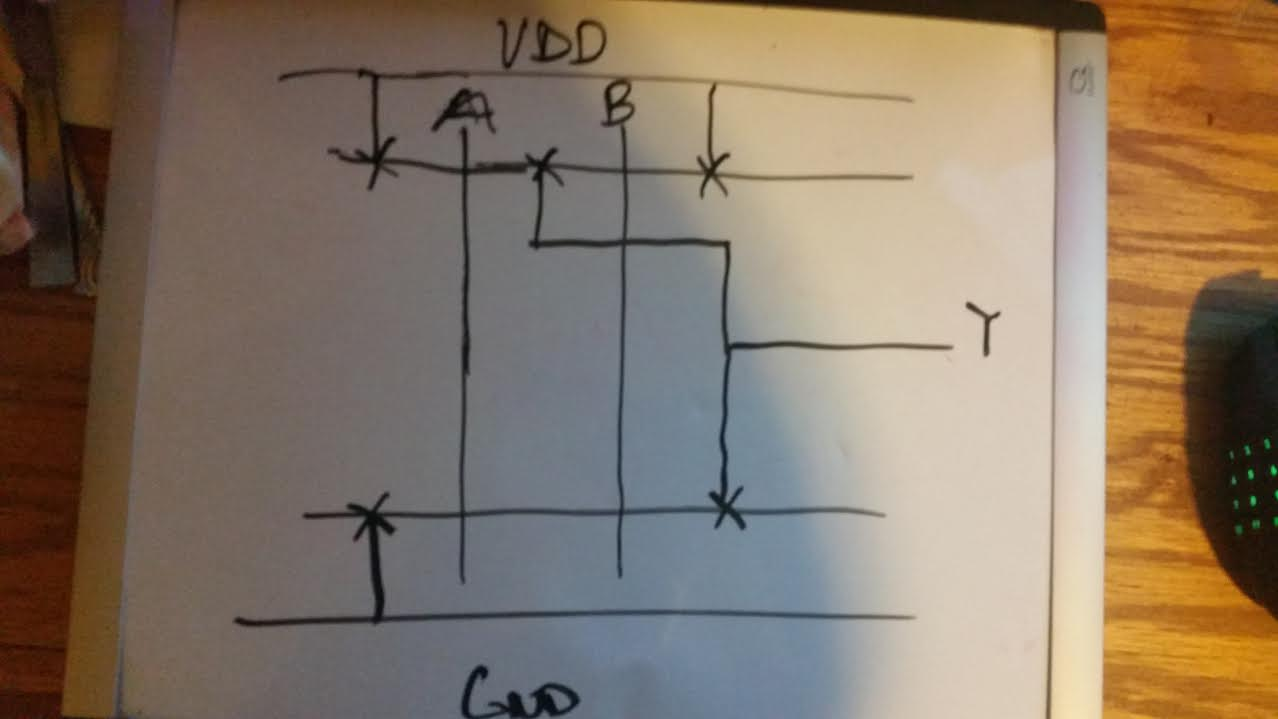
\includegraphics[width=0.7\linewidth]{prelab-stick}
\caption{Stick Digram for Static CMOS 2-input NAND Gate}
\label{fig:prelab-stick}
\end{figure}

\begin{figure}[H]
\centering
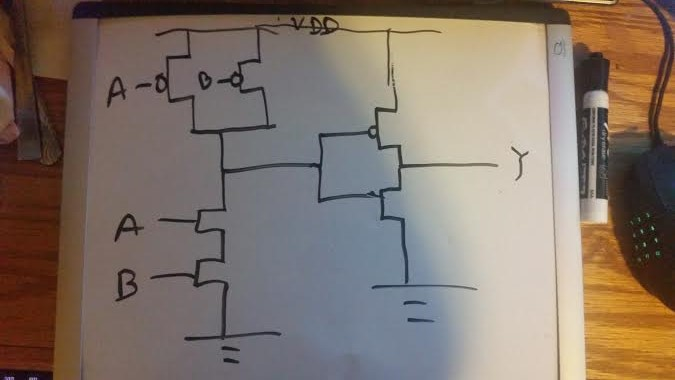
\includegraphics[width=0.7\linewidth]{prelab-design}
\caption{2-input AND Gate Design}
\label{fig:prelab-design}
\end{figure}

\section{Implementation}
\subsection{Schematics}
\begin{figure}[H]
	\centering
	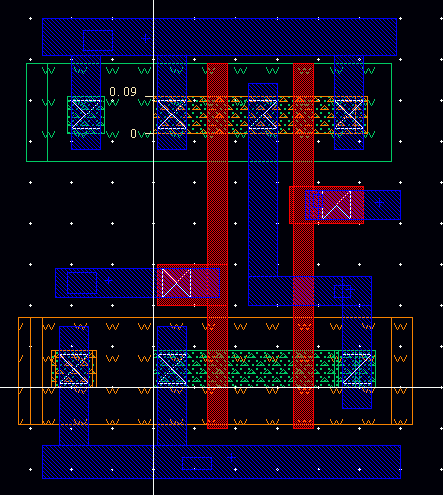
\includegraphics[width=\linewidth]{nand2-layout}
	\caption{2-input NAND Gate Layout}
	\label{fig:nand2-layout}
\end{figure}

\begin{figure}[H]
\centering
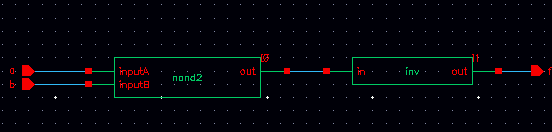
\includegraphics[width=\linewidth]{and2-schematic}
\caption{2-input And Gate Schematic}
\label{fig:and2-schematic}
\end{figure}

\begin{figure}[H]
\centering
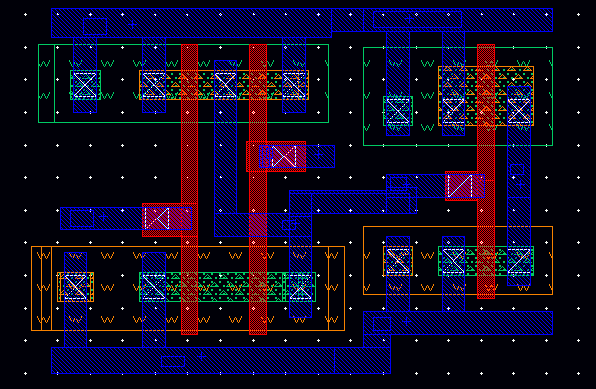
\includegraphics[width=\linewidth]{and2-layout}
\caption{2-input AND Gate Layout}
\label{fig:and2-layout}
\end{figure}


\begin{figure}
\centering
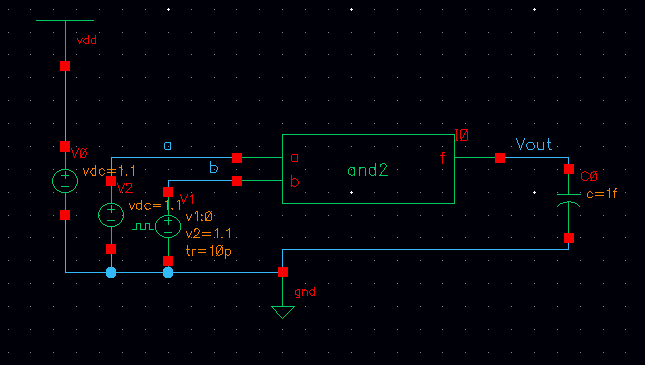
\includegraphics[width=\linewidth]{and2-test-circuit}
\caption{Test Circuit for 2-input AND Gate}
\label{fig:and2-test-circuit}
\end{figure}



\subsection{Procedure}
A NAND gate  layout was created in Virtuoso and was verified using LVS. After this, a 2-input AND gate was designed using both the schematic and layout view. This was then verified using LVS, and it was also verified against the verilog model. Delay was then calculated for the AND gate design.
\subsection{Results}
\begin{figure}[H]
\centering
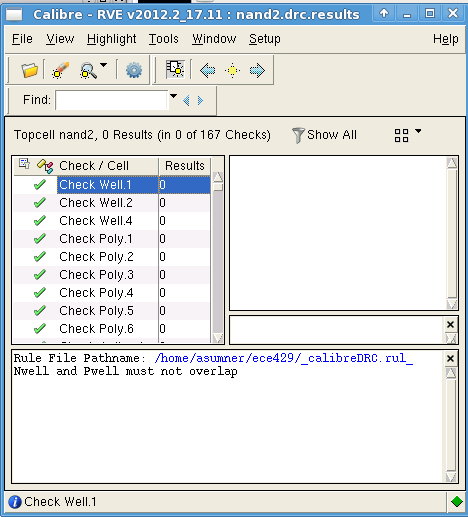
\includegraphics[width=0.7\linewidth]{drc-nand2}
\caption{2-input NAND Gate DRC Results}
\label{fig:drc-nand2}
\end{figure}

\begin{figure}[H]
\centering
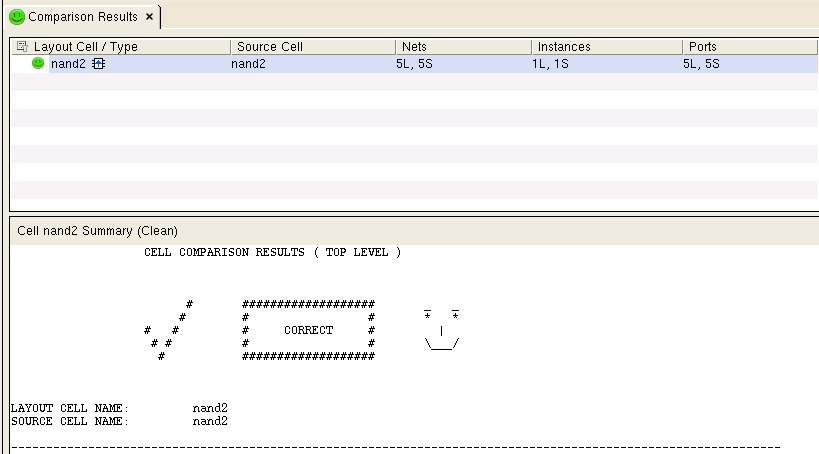
\includegraphics[width=0.7\linewidth]{nand2-lvs}
\caption{2-input NAND Gate LVS Results}
\label{fig:nand2-lvs}
\end{figure}

\begin{figure}[H]
\centering
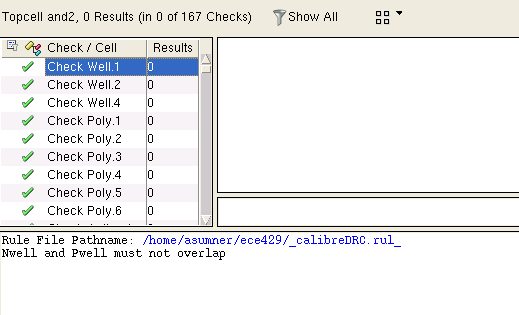
\includegraphics[width=0.7\linewidth]{and2-drc}
\caption{2-input AND Gate DRC Results}
\label{fig:and2-drc}
\end{figure}

\begin{figure}[H]
\centering
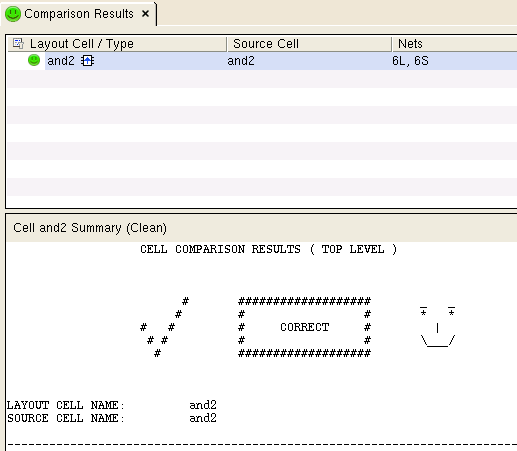
\includegraphics[width=0.7\linewidth]{and2-lvs}
\caption{2-input AND Gate LVS Results}
\label{fig:and2-lvs}
\end{figure}


\begin{figure}[H]
\centering
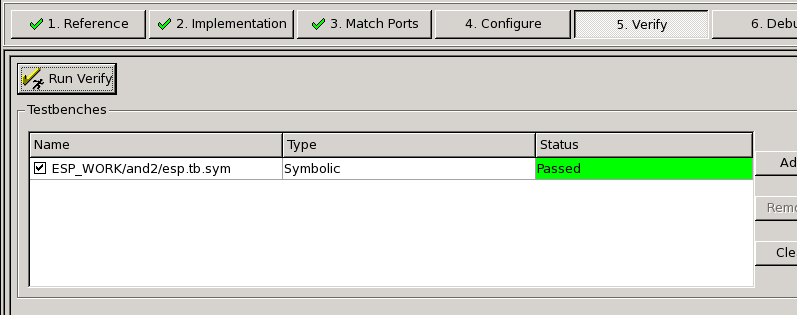
\includegraphics[width=0.7\linewidth]{verilog-verified}
\caption{Verilog Equivalence Validated}
\label{fig:verilog-verified}
\end{figure}


\begin{figure}
\centering
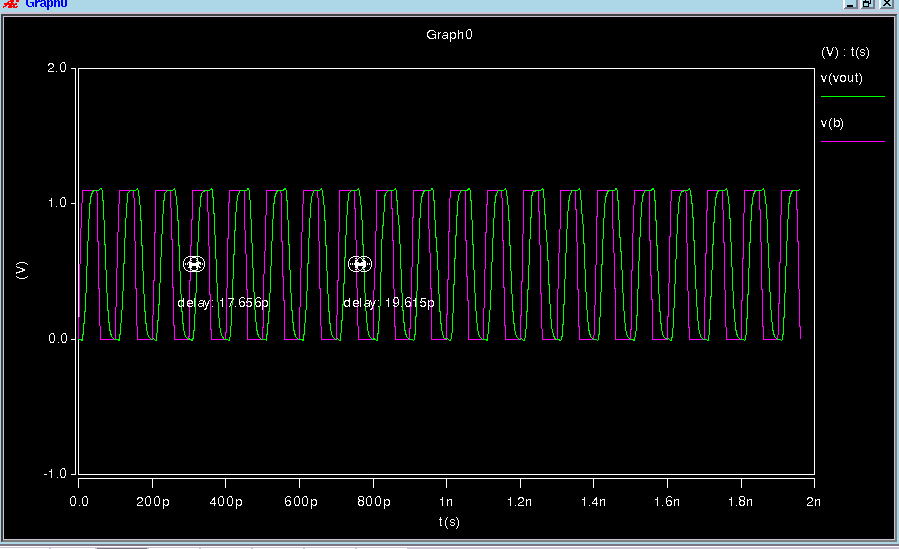
\includegraphics[width=\linewidth]{10-11-delay}
\caption{10 $\to$ 11 Delay Measurements}
\label{fig:10-11-delay}
\end{figure}

\begin{figure}[H]
\centering
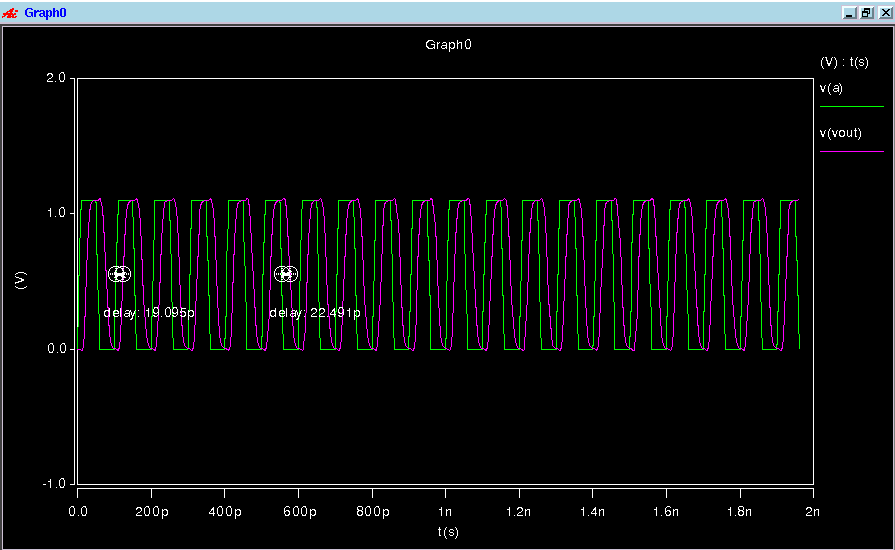
\includegraphics[width=\linewidth]{01-11-delay}
\caption{01 $\to$ 11 Delay Measurements}
\label{fig:01-11-delay}
\end{figure}


\begin{figure}
\centering
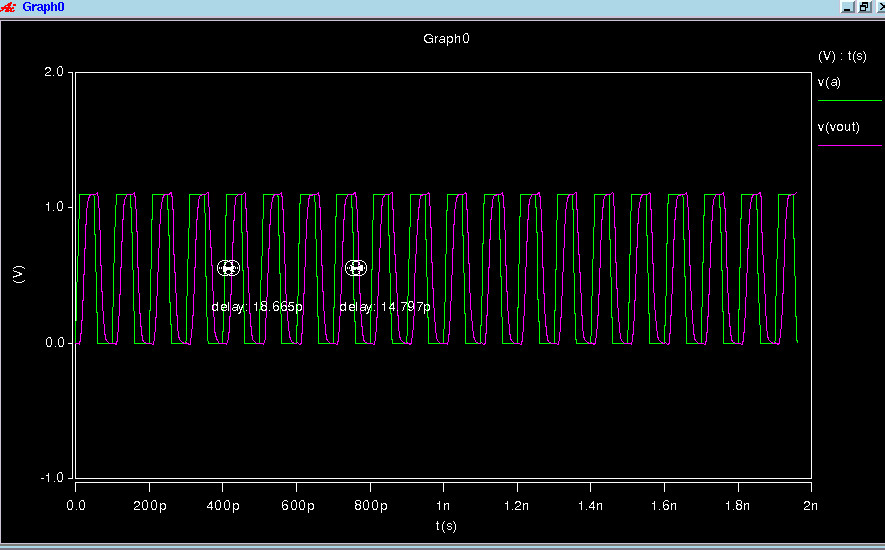
\includegraphics[width=\linewidth]{00-11-delay}
\caption{00 $\to$ 11 Delay Measurements}
\label{fig:00-11-delay}
\end{figure}

\begin{table}[H]
	\begin{center}
		\begin{tabular}{ |c|c|c|c| }
			\hline
			w=90nm &
			\multicolumn{3}{|c|}{Transition} \\
			\cline{2-4} l=50nm & 10$\to$11 & 01$\to$11 & 00$\to$11 \\
			\hline
			Rising Propogation Delay & 17.656e-12 s & 19.095e-12 s & 18.665e-11 s  \\
			\hline
			Falling Propogation Delay & 19.615e-11 s& 22.491e-11 s& 14.797e-11 s\\
			\hline
			Average Power Consumption & 3.17-05 W& 3.26e-05 W& 3.23e-05 W\\
			\hline
		\end{tabular}
	\end{center}
	\caption{Delay and Power Consumption of Each Excition with 1f Load Capacitance}
	\label{tab:1st}
\end{table}

\subsection{Discussion}

\subsection{Questions}
	
%\subsection{Bonus Work}
\section{Conclusions}

\end{document}
